\documentclass{article}

\usepackage{microtype}
\usepackage{graphicx}
\graphicspath{{figures/}{./}}
\usepackage{booktabs}
\usepackage{amsmath,amssymb,mathtools}
\usepackage{hyperref}
\usepackage[preprint]{styles/icml2026}
\usepackage[capitalize,noabbrev]{cleveref}
\hypersetup{pdfsubject={Working preprint}}

\icmltitlerunning{Token Cramming through Shared Prediction Embeddings}
\newcommand{\R}{\mathbb{R}}
\newcommand{\CE}{\mathcal{L}_{\mathrm{CE}}}
\newcommand{\MH}{\mathcal{L}_{\mathrm{margin}}}
\newcommand{\sg}{\mathrm{sg}}
\newcommand{\sourcecommit}[1]{{\small\texttt{#1}}}

\begin{document}

\twocolumn[
  \icmltitle{Token Cramming through Shared Prediction Embeddings}
  % Author metadata is inherited from the repository's earlier working draft.
  \begin{icmlauthorlist}
    \icmlauthor{Dmitrii Tarasov}{fusionbrain,hse}
    \icmlauthor{Timofei Lashukov}{hse}
    \icmlauthor{Elizaveta Goncharova}{fusionbrain,hse}
    \icmlauthor{Andrey Kuznetsov}{fusionbrain,innopolis}
  \end{icmlauthorlist}
  \icmlaffiliation{fusionbrain}{FusionBrain Lab, Moscow, Russia}
  \icmlaffiliation{hse}{HSE University, Moscow, Russia}
  \icmlaffiliation{innopolis}{Artificial Intelligence Institute, Innopolis University, Innopolis, Russia}
  \icmlcorrespondingauthor{Dmitrii Tarasov}{dtarasov@hse.ru}
  \icmlkeywords{token cramming, continuous conditioning, exact reconstruction, transformer mechanisms}
  \vskip 0.3in
]
\printAffiliationsAndNotice{}

\begin{abstract}
How much text a frozen transformer reconstructs from one learned vector depends on how that vector enters the computation.
We study progressive token cramming in matched Standard and SPS checkpoints, where SPS separates ordinary input positions from prediction positions.
Within the same frozen SPS checkpoint, replacing an ordinary memory token with a fixed beginning-of-sequence token and learning one vector shared across prediction inputs raises mean exact teacher-forced length from 31.52 to 132.10 tokens on 48 matched texts under a strict margin objective, using the same 768 trainable scalars.
Cross-entropy also benefits, from 19.42 to 64.17 tokens, and random initialization gives a similar margin-objective result.
The vector is reused at every prediction position, so equal parameter count does not equate the conditioning interfaces.
An extended-budget control that preserves the original learning-rate trajectory reaches 133.85 tokens and stops on a local stage limit in every text; stretching the schedule instead reaches 79.42.
Older ordinary-memory interventions reveal context-mediated and direct prediction routes, while local rescues demonstrate that some failed prefixes remain feasible.
These findings establish a large conditioning-site effect in one checkpoint, while leaving architecture attribution, a global capacity ceiling, and guaranteed exact free generation unresolved.
\end{abstract}

\section{Introduction}
\label{sec:intro}

Token cramming optimizes a small continuous input separately for each text while keeping the language model frozen \citep{kuratov2025cramming}.
The resulting reconstruction length is a property of a text, a decoder, a conditioning interface, and an optimization procedure.
It is tempting to interpret a failed reconstruction stage as the point at which an embedding runs out of capacity.
That interpretation requires more than observing that one finite optimization run stopped.
The same vector dimension may support substantially different reconstruction when its computational access changes.

We investigate this issue using two native checkpoints: a conventional causal transformer, called \emph{Standard}, and an SPS transformer with interleaved ordinary input and prediction slots.
At the zero prediction window studied here, earlier prediction states cannot be read by subsequent positions.
This creates a useful distinction between controlling an ordinary memory position and controlling the prediction stream itself.
An ordinary memory can influence both later ordinary context states and prediction states through attention.
A vector shared only across prediction inputs directly changes readout computations while leaving ordinary context states independent of that vector for a fixed token history.

Our central experiment holds the SPS checkpoint, texts, vector dimension, and progressive protocol fixed while changing this conditioning interface.
With a strict margin objective, mean selected teacher-forced length increases from 31.52 to 132.10 tokens.
Every one of the 48 texts improves.
The corresponding Standard ordinary-memory result is 54.83 tokens, but that comparison does not isolate architecture: the checkpoints have different learned weights, and Standard has not received an analogous repeatedly applied readout intervention.
The most direct conclusion is therefore within-checkpoint: the earlier SPS ordinary-memory result is not a ceiling on this checkpoint's ability to reconstruct from one learned vector.

We also examine what the achieved lengths measure.
A matched objective factorial shows that a margin loss helps both ordinary-memory models without removing the Standard--SPS gap.
A larger-budget study separates available updates from the learning-rate trajectory and actual updates used.
The restored trajectory adds only 1.75 tokens on average before all texts hit the per-stage limit.
At those terminal stages, multiple positive-margin constraints fail, including previously satisfied constraints.
These are not necessarily argmax errors.
Finally, interventions and local geometry probes on the earlier ordinary-memory protocol identify causal routes and recover several failed prefixes without changing the model or vector size.
We keep those findings separate from the much longer shared-prediction frontier.

The study makes three contributions: a controlled change of conditioning site with a large same-checkpoint gain; objective, schedule, stopping, and free-generation measurements that bound the interpretation of that gain; and a reproducibility bundle that rebuilds the reported evidence without running new optimization.
All claims concern the measured checkpoints and matched texts rather than an architecture-wide capacity law.

\section{Related Work}
\label{sec:related}

\paragraph{Per-text continuous reconstruction.}
\citet{kuratov2025cramming} replace an encoder with per-sample optimization and demonstrate reconstruction from highly compressed continuous inputs.
They argue that uncertainty reduction, rather than raw sequence length alone, better characterizes the limits they observe.
We use token length as an operational measure on a fixed text cohort and decoder; we do not interpret it as a decoder-independent stored-bit count.
Our question concerns the conditioning interface and the distinction between achieved reconstruction and infeasibility.

\paragraph{Continuous conditioning of frozen models.}
Prefix tuning learns continuous task-specific prefixes while keeping the language model frozen \citep{li2021prefix}.
Prompt tuning similarly optimizes soft prompts for downstream tasks \citep{lester2021power}.
Here the learned vector is text-specific, and the criterion is reconstruction of that text rather than generalization to a task distribution.
Our shared-prediction intervention also differs computationally from placing one learned token before a sequence: its parameters are tied across all prediction inputs.
These distinctions matter when comparing the number of learned scalars or interpreting semantic utility.

\paragraph{Attention routes and controllability.}
The separation of query--key addressing from output--value transmission in the transformer-circuits framework motivates our key/value interventions \citep{elhage2021mathematical}.
That framework's attention-only examples do not establish mechanisms in our deeper models with MLPs.
We therefore measure counterfactual effects directly and avoid treating attention weights, intervention effects, or local Jacobian rank as an additive capacity decomposition.

\section{Reconstruction and Conditioning Interfaces}
\label{sec:method}

\subsection{Progressive feasibility}

For a text prefix $x_{1:L}$ and a learned vector $z\in\R^d$, let
$\ell_t(z;x_{<t})\in\R^{|\mathcal V|}$ denote the target-aligned logits of the frozen decoder.
Define the target-versus-best-rival gap
\begin{equation}
 m_t(z)=\ell_{t,x_t}(z)-\max_{v\ne x_t}\ell_{t,v}(z).
 \label{eq:margin}
\end{equation}
Exact teacher forcing requires the target to be the selected argmax at every position.
Strict convergence additionally requires $m_t\ge\epsilon$ for every target.
We optimize either mean cross-entropy or a squared margin deficit,
\begin{align}
 \CE(z)&=-\frac{1}{L}\sum_{t=1}^{L}\log p_z(x_t\mid x_{<t}),\\
 \MH(z)&=\frac{1}{L}\sum_{t=1}^{L}[\tau-m_t(z)]_+^2.
 \label{eq:objective}
\end{align}
The loss target $\tau$ and stopping gap $\epsilon$ are separate controls.
In the strict-hinge comparisons both are 0.05.
The reported raw criterion uses argmax matching without a positive stopping gap.

Progressive optimization begins with one target and extends the prefix by one token after convergence.
The learned vector and optimizer state are inherited across stages.
The \emph{teacher-forced horizon} $H$ is the length of the deepest converged saved stage under the registered budget.
It is an achieved length, not a proof that length $H+1$ is infeasible.
We select one final converged vector per text and evaluate its full teacher replay and greedy decoding separately.
The \emph{initial correct greedy prefix} $G$ counts generated tokens before the first error for that vector, up to its selected length $H$.
We do not search earlier vectors for a better greedy result.

\subsection{Native Standard and zero-window SPS}
\label{sec:sps}

Standard uses an ordinary causal sequence $[c_0,c_1,\ldots]$.
For ordinary-memory cramming, $c_0=z$ and $c_j=E(x_j)$ for $j\ge1$; the output at position $t-1$ predicts $x_t$.
SPS interleaves each ordinary input with a prediction input,
\begin{equation}
 [c_0,p_0,c_1,p_1,\ldots,c_L,p_L],
 \label{eq:interleave}
\end{equation}
where $c_j$ and $p_j$ share rotary position $j$, and output logits are read only at $p_j$.
For interleaved query and key indices $q,k$, the zero-window visibility rule is
\begin{equation}
 A_{qk}=\mathbf{1}\{k\le q\}\,
 \mathbf{1}\{k\text{ even}\ \lor\ \lfloor q/2\rfloor=\lfloor k/2\rfloor\}.
 \label{eq:mask}
\end{equation}
Thus ordinary keys persist, while a prediction slot can read its own temporary key/value but earlier prediction keys expire.
Ordinary states cannot read any prediction slot.
The first target is read from $p_0$, after the initial ordinary slot; BOS is not a reconstructed target.

In ordinary-memory SPS, $c_0=z$ and every $p_j$ begins at the frozen native prediction embedding $e_{\mathrm{pred}}$.
The initial memory state is causally autonomous: its layerwise trajectory depends on itself, while other positions may read its outgoing keys and values.
Later ordinary states can consequently depend on $z$ despite input/prediction separation.

In \emph{shared-prediction cramming}, we set $c_0=E(\mathrm{BOS})$ and $p_j=z$ at every prediction input.
The same $d$ scalars are reused rather than learning $L$ separate vectors.
By \cref{eq:mask}, the ordinary context states are independent of $z$ at every layer conditional on a fixed token history.
During free generation the chosen history itself can depend on $z$.
Each prediction state receives direct residual input, query control, and its own temporary key/value through $z$, which can also affect its subsequent MLP computation.
This changes several routes together; it does not isolate which one causes the gain.
We replace prediction \emph{inputs} only: the tied output head and its prediction-token row stay frozen, and no vocabulary item is added.

\subsection{Matched measurements and numerical regime}

The main cohort consists of the same 48 cached PG-19 texts selected by the source registry, with GPT-2 tokenization and exact target-ID matching across arms.
Both checkpoints have 12 layers and hidden width 768 and were saved after 1,000,341,504 training tokens.
The run label \texttt{pilot\_1b} refers to the pretraining token budget.
All full progressive cramming runs use one vector and batch size one, frozen weights, and BF16 model arithmetic.
The main comparisons use an initial learning rate of 0.3, at most 10,000 updates per text, and at most 1,000 updates at a new stage.
The code registries remain the design authority; \cref{app:repro} maps each measurement to its source.

Reported intervals resample matched texts as pairs at fixed checkpoints and a fixed optimization seed.
They describe variation over this text cohort, not checkpoint, pretraining-seed, or optimization-seed uncertainty.
Free generation uses the same BF16 checkpoint and learned vector as training, with the ordinary generated history and native SPS mask.
Teacher replay and incremental decoding can differ numerically because the forward context shape changes.
We consequently report observed greedy outcomes rather than inferring them from teacher-forced success.

\section{The Conditioning Site Changes Achieved Length}
\label{sec:site}

\begin{table*}[t]
 \centering
 \small
 % Generated by sps_paper/reproduce.py; edit measurements or generator.
\begin{tabular}{lrrrrr}
\toprule
Model / site & Objective / stop & TF horizon [95\% CI] & Exact & Initial prefix & Updates \\
\midrule
Standard / memory & CE / argmax & 32.31 [30.90, 33.73] & 48/48 & 32.31 & 2382 \\
Standard / memory & Hinge / margin & 54.83 [52.06, 57.73] & 44/48 & 52.50 & 5407 \\
SPS / memory & CE / argmax & 19.42 [18.29, 20.56] & 46/48 & 19.06 & 1769 \\
SPS / memory & Hinge / margin & 31.52 [29.94, 33.15] & 45/48 & 30.56 & 2620 \\
SPS / predict (native) & CE / argmax & 64.17 [60.96, 67.29] & 37/48 & 56.52 & 3460 \\
SPS / predict (native) & Hinge / margin & 132.10 [127.81, 136.46] & 38/48 & 110.23 & 9891 \\
SPS / predict (random) & Hinge / margin & 130.23 [124.17, 135.77] & 43/48 & 118.65 & 9632 \\
\bottomrule
\end{tabular}

 \caption{Matched original-budget reconstruction results. $H$ is the selected exact teacher-forced length; $G$ is the initial correct greedy prefix of that selected vector. Exact greedy counts concern each arm's own selected length. Every selected vector replays exactly under teacher forcing. All arms learn 768 scalars per text.}
 \label{tab:main}
\end{table*}

\begin{figure}[t]
 \centering
 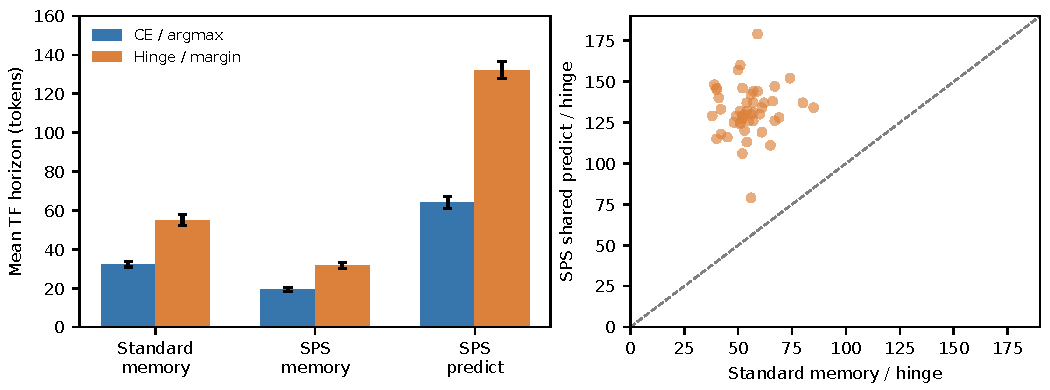
\includegraphics[width=\columnwidth]{site_objective.pdf}
 \caption{Achieved teacher-forced lengths under the original matched budget. The large within-SPS change comes from conditioning the prediction inputs with one shared vector. The Standard comparison also changes the learned checkpoint.}
 \label{fig:site}
\end{figure}

Within SPS, shared-prediction conditioning raises mean $H$ from 19.42 to 64.17 under CE and from 31.52 to 132.10 under strict hinge (\cref{tab:main,fig:site}).
The paired gains are 44.75 tokens (95\% text-bootstrap interval 41.50--47.98) and 100.58 (96.46--104.60), respectively.
Every text improves in both comparisons.
The strict-hinge mean is approximately 4.2 times the ordinary-memory mean for the same checkpoint and vector dimension.

The effect does not require initialization at the pretrained prediction row.
Random-initialized shared-prediction hinge reaches 130.23 tokens, a gain of 98.71 (93.00--103.96) over the ordinary-memory control.
Native minus random initialization is only 1.88 tokens, with interval $-2.23$--6.04; these runs establish no winner between the two initializations.
All three shared-prediction arms improve teacher-forced length on all 48 texts relative to their corresponding ordinary-memory control.

Longer teacher-forced prefixes remain less reliable under free generation.
The native hinge arm has mean $G=110.23$ and exactly reconstructs 38/48 selected prefixes, compared with $G=30.56$ and 45/48 for ordinary-memory strict hinge.
The random arm has $G=118.65$ and 43/48 exact selected prefixes.
These counts compare different lengths; they do not show a matched-length robustness ranking.
In particular, the 132.10 mean teacher-forced length is not a guaranteed lossless greedy horizon.

What has changed is the access provided to one text-specific vector.
Ordinary memory supplies one causal position's outgoing layerwise keys and values, with effects relayed through the context.
Shared prediction instead supplies the initial residual state of each readout position while ordinary states remain independent of that vector conditional on the token history.
The same vector can yield different tokens because position and reconstructed history differ.
Equal scalar count therefore controls the number of learned parameters, but not intervention sites, attention computation, or forward cost.

\section{Objectives and Optimization Limits}
\label{sec:controls}

\subsection{Exact constraints and mean cross-entropy}

The ordinary-memory objective factorial crosses CE versus squared hinge with raw versus strict stopping (\cref{tab:factorial}).
Raw CE reaches 32.31 tokens for Standard and 19.42 for SPS.
Strict hinge raises these to 54.83 and 31.52: gains of 22.52 (19.79--25.31) and 12.10 (10.46--13.79).
Changing the loss helps both checkpoints substantially, while the absolute Standard-minus-SPS gap increases from 12.90 to 23.31 tokens.
Under raw stopping, proportional gains are also similar (77.8\% and 81.2\%).
Loss choice is a shared bottleneck rather than an explanation that removes the SPS disadvantage.

The positive stopping gap has a separate role.
For hinge, it reduces selected lengths from 57.46 to 54.83 for Standard and 35.19 to 31.52 for SPS, while exact greedy counts increase from 37/48 to 44/48 and 29/48 to 45/48.
The two objectives should therefore be compared with their stopping criteria identified.
Even strict convergence does not guarantee exact BF16 decoding.

A local audit of four selected failed SPS ordinary-memory prefixes explains one way CE can be poorly aligned with feasibility.
Exact hinge solutions have higher mean CE than their corresponding erroneous CE-restart vectors in every case (3.181 versus 1.209 averaged across cases).
At each selected CE vector, correct- and wrong-token CE gradients oppose one another, and infinitesimal plain CE descent worsens the worst-token margin.
This establishes a local mismatch, not a statement about global CE minima or the direction of the actual preconditioned, momentum-bearing Adam step.

\subsection{Available budget is not used budget}
\label{sec:budget}

\begin{table*}[t]
 \centering
 \small
 % Generated by sps_paper/reproduce.py; edit measurements or generator.
\begin{tabular}{lrrrrr}
\toprule
Schedule & TF horizon [95\% CI] & Initial prefix & Exact & Budget stop & Stage stop \\
\midrule
Original & 132.10 [127.81, 136.46] & 110.23 & 38/48 & 47 & 1 \\
Stretched LR & 79.42 [76.60, 82.23] & 76.12 & 44/48 & 0 & 48 \\
Fixed LR + floor & 133.85 [129.44, 138.31] & 121.19 & 41/48 & 0 & 48 \\
\bottomrule
\end{tabular}

 \caption{Native-initialized shared-prediction strict hinge under three completed protocols. The extension allows more total updates; its fixed-schedule version preserves the original learning-rate path and then holds its endpoint. Exact greedy counts concern different selected lengths.}
 \label{tab:budget}
\end{table*}

\begin{figure}[t]
 \centering
 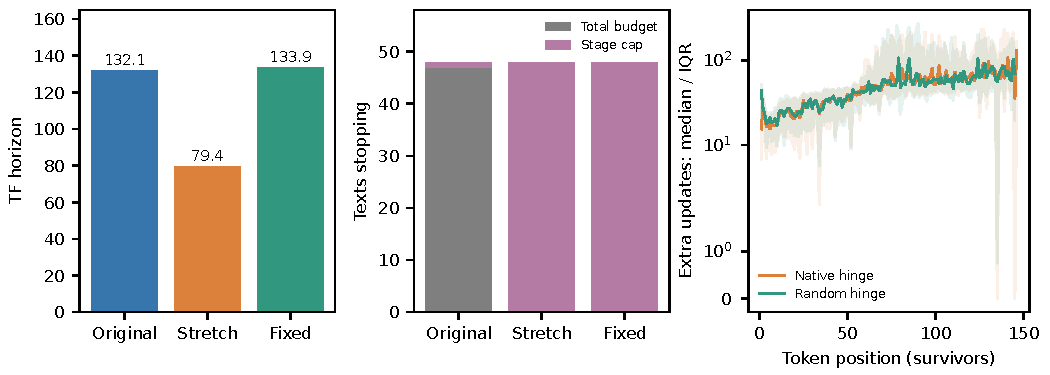
\includegraphics[width=\columnwidth]{budget_control.pdf}
 \caption{Shared-prediction budget control. Preserving the original learning-rate trajectory recovers the regression caused by stretching it. The extended run stops at local stage failures before exhausting the larger total budget.}
 \label{fig:budget}
\end{figure}

The original native-hinge run reaches the total update limit on 47/48 texts, suggesting budget censoring.
Simply raising the available total budget to 30,000 also stretches the existing cosine learning-rate schedule.
That completed protocol reaches only 79.42 tokens, with every text worse and every run stopping at a stage failure before using the total budget.
It does not isolate the effect of extra updates.

We therefore compare it with a fresh deterministic replay that allows the same extended budget but fixes the original learning-rate trajectory, holding its endpoint after the original scheduler horizon.
The fixed-trajectory result is 133.85 tokens (\cref{tab:budget,fig:budget}).
All 48 texts improve relative to the stretched schedule, by 54.44 tokens on average (50.65--58.06).
Relative to the original run, 33 improve, 15 tie, and none worsen; mean gain is 1.75 (1.19--2.40), about 1.3\%.
All 6,342 paired stages ending before the original budget boundary match exactly in optimized vector, update count, and convergence flag.
This supports the learning-rate intervention as the explanation of the stretched-schedule regression in this matched comparison.

The extended fixed-trajectory runs use 11,391.65 updates per text on average (range 4,784--15,082), versus 9,891.33 originally.
Every one stops after a failed stage's 1,000-update allowance; none reaches 30,000.
The available total budget tripled, but actual mean updates increased by about 15.2\% and teacher-forced length by 1.3\%.
This is evidence of a remaining protocol limit, not a global representational ceiling.
Mean $G$ rises to 121.19 with 41/48 exact selected prefixes, but the paired greedy-prefix gain interval includes zero ($-3.42$--25.35).

\subsection{Terminal failure involves old constraints}
\label{sec:terminal}

\begin{figure}[t]
 \centering
 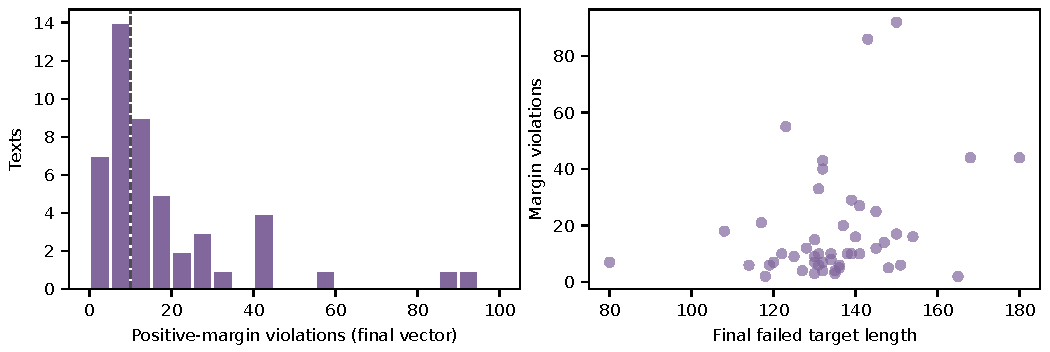
\includegraphics[width=\columnwidth]{terminal_constraints.pdf}
 \caption{Positive-margin violations at the first failed stage of the extended fixed-trajectory run. Every stage adds one target to a previously converged prefix. Counts above one necessarily include old target constraints, but do not identify argmax errors or their cause.}
 \label{fig:terminal}
\end{figure}

The saved-stage terminal audit counts violations of the recorded positive-margin stopping criterion rather than only a failed-stage flag.
The median is ten constraints, with range two to 92; the equal-text mean fraction satisfying the margin is 87.08\% (\cref{fig:terminal,tab:terminal}).
Every preceding stage converged, and each terminal stage adds exactly one target.
Consequently every terminal failure violates at least one old target constraint; the median lower bound is nine old-position violations.
This rules out describing the saved failure solely as inability to fit the new target while preserving all earlier margins.

The audit does not record a positionwise before/after replay.
It cannot determine which old positions fail, whether their argmax changes, or how much failure comes from optimization versus BF16 changes induced by the longer context shape.
A target can remain the argmax and still miss the 0.05 gap.
Separating these causes requires per-position replay under controlled arithmetic and the same quantized weights.

\section{Mechanism Evidence from Ordinary Memory}
\label{sec:mechanism}

The following interventions concern the earlier ordinary-memory protocol, at short matched prefixes or its first failed stages.
They do not diagnose the longer shared-prediction frontier.
Their role is to test simple explanations of ordinary-memory behavior and clarify why the site intervention changes the causal picture.

\subsection{Context mediation and direct prediction reads}

\begin{figure}[t]
 \centering
 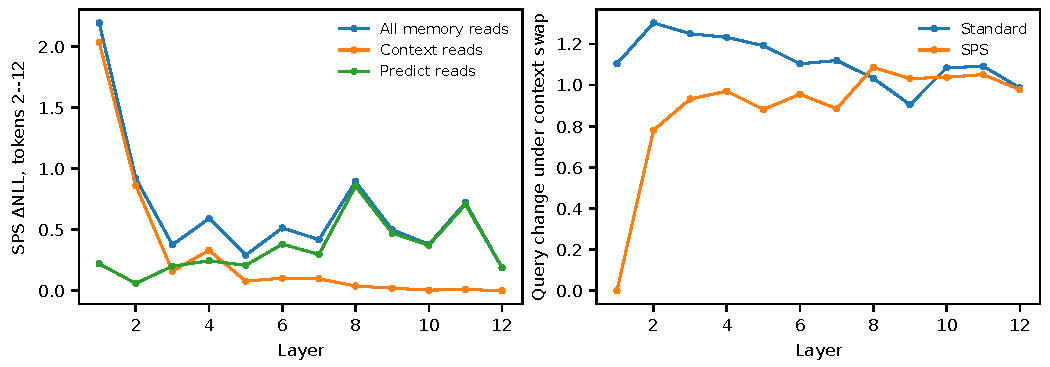
\includegraphics[width=\columnwidth]{routes.pdf}
 \caption{Ordinary-memory route interventions at matched exact prefixes. SPS has a strong early memory-to-context effect and stronger later direct memory-to-prediction effect. These counterfactual NLL changes are non-additive and do not measure shared-prediction capacity.}
 \label{fig:routes}
\end{figure}

We remove selected attention edges from the memory key, renormalizing the remaining attention, and distinguish destinations in ordinary context versus prediction slots.
At matched exact-stage memories, first-layer SPS memory-to-context knockout increases NLL by 2.034 nats/token, versus 0.220 for memory-to-prediction knockout; the joint effect is 2.194.
By layer eight the effects are 0.038 and 0.857, respectively (\cref{fig:routes,tab:routes}).
Thus a fixed, context-independent initial prediction query does not imply that the dominant early memory effect is a direct prediction read.
Memory information can first modify ordinary context states and be read later.

A complementary intervention replaces projected memory keys or values with those produced by a norm-matched donor memory while retaining the original memory residual trajectory.
Across layers, donor-value replacement increases NLL by 5.277 for Standard and 4.834 for SPS; donor-key replacement gives 2.396 and 2.450.
Self-patching is an identity control to within $3.70\times10^{-6}$ NLL, and joint all-layer key/value patching reproduces the donor-memory condition on scored positions.
Values have the larger effect under this intervention in both models.
These effects neither count stored bits nor sum to independent route contributions.
We exclude the first target from scored route comparisons because Standard predicts it directly from the memory residual.

\subsection{Local rank and unchanged-dimension rescues}
\label{sec:geometry}

At the first failed SPS ordinary-memory length, we differentiate the margins in \cref{eq:margin} with respect to the learned memory vector and compare both checkpoints at the same target length.
Every measured previous-token margin Jacobian has full row rank.
At warm start, the mean fraction of the new-token gradient orthogonal to previous-token constraint rows is 0.847 for Standard and 0.875 for SPS.
These results weaken a simple local rank-exhaustion explanation.
They do not guarantee a finite feasible step: the active competitor may change, nonlinear curvature matters, and protected old margins can fail after a finite perturbation.
Moreover, SPS is evaluated at its own frontier whereas Standard is usually below its frontier.

Restarting four selected failed SPS prefixes without changing the checkpoint or memory dimension supplies a more direct feasibility test (\cref{tab:rescue}).
CE restarts recover none within the diagnostic budget.
Squared-margin Adam recovers all four in FP32, and three pass both exact teacher replay and greedy generation in the original BF16 regime.
A constrained margin controller also recovers all four in FP32, with only one passing BF16 validation.
The three original-precision successes disprove infeasibility at those selected original stopping points.
They do not establish a new progressive horizon, remove the overall Standard--SPS gap, or transfer automatically to shared-prediction failures.

\section{Discussion and Limitations}
\label{sec:discussion}

The central result is that conditioning the shared SPS prediction input substantially improves achieved reconstruction for this frozen checkpoint.
An ordinary memory's horizon therefore cannot be read as the intrinsic capacity of a 768-dimensional control vector.
The accessible route matters: ordinary-memory information reaches prediction computations through outgoing memory keys/values and context mediation, whereas shared prediction directly initializes each readout state.
Avoiding modifications to ordinary context may reduce interference, but that hypothesis remains unisolated from query, residual, and temporary self-key/value effects.
All prediction constraints still share the same vector, and the terminal audit shows that old constraints can fail together with the new one.

Three comparisons must remain distinct.
First, the conditioning-site comparison holds one SPS checkpoint fixed and demonstrates a large protocol effect.
Second, the ordinary-memory Standard--SPS comparison changes learned weights as well as architecture.
Third, the extended-budget comparison changes optimization opportunity and, unless explicitly fixed, its schedule.
None is an architecture-only or parameter-count-only capacity experiment.
Repeated intervention sites and SPS's interleaved forward computation also prevent an efficiency claim based only on learned scalar count.
The comparisons do not match FLOPs or wall-clock time; SPS doubles the internal positions relative to its ordinary input sequence.

The evidence is restricted to one checkpoint of each type, 48 matched texts, and one optimization seed.
Bootstrap intervals quantify text variation only; initialization and schedule comparisons are selected finite experiments rather than a resolved optimum.
The native/random comparison supports similar achieved lengths within uncertainty, not initialization invariance in general.
Local route and geometry measurements describe their selected states, not all solutions.
We do not measure semantic transfer, downstream usefulness, or decoder-independent representation quality for the new vectors.

Finally, exact teacher replay is distinct from reliable compression for free generation.
Several selected long prefixes fail greedy decoding despite a positive training margin.
Observed stopping also remains a finite optimization outcome: the final fixed-trajectory experiment exhausts its local stage allowance before its total budget.
An analogous repeatedly applied Standard readout intervention, route isolation within shared prediction, and controlled per-position replay at its failed stages would distinguish remaining causal explanations.
Successful rescues would establish feasibility for particular prefixes; unsuccessful searches would still not certify a global ceiling.

\section{Conclusion}

One shared prediction-input vector raises the SPS checkpoint's original-budget mean exact teacher-forced reconstruction from 31.52 to 132.10 tokens while retaining 768 learned scalars per text.
The effect persists under CE and with random initialization.
Objective and schedule controls show that achieved horizons also depend materially on optimization, and older same-dimension rescues demonstrate that failure need not imply infeasibility.
The supported claim is a large improvement in a particular conditioning protocol, with free-generation reliability and architecture-level capacity left open.

\bibliography{references}
\bibliographystyle{styles/icml2026}

\appendix
\section{Reproducibility and Evidence Boundaries}
\label{app:repro}

The manuscript accompanies an independent reproducibility bundle in \texttt{sps\_paper/}; it does not modify the earlier \texttt{paper/} draft.
The bundle distinguishes three operations.
\emph{Export} reads completed experiment artifacts and validates the compact evidence snapshot.
\emph{Render} rebuilds the paper's tables and figures from the versioned snapshot without checkpoints, a GPU, shared storage, or network access.
\emph{Plan} describes historical experiment replay and its external prerequisites; it does not submit a job.
Rebuilding a figure is consequently distinct from rerunning the optimization that produced its observations.
The snapshot is stored in \path{data/manifest.json},
\path{data/cohort.json.gz}, \path{data/runs.json.gz}, and
\path{data/probes.json.gz}; \path{data/derived_metrics.json} records the computed summaries.
From the repository root, offline rendering uses
\texttt{python sps\_paper/reproduce.py render}; the nonexecuting historical replay plan uses
\texttt{python sps\_paper/reproduce.py plan}.
The accompanying README records the remaining commands, and the snapshot records complete source commits and full job identifiers.

\paragraph{Design authority.}
Experiment design lives in the Python registries, rather than this manuscript's descriptive summaries.
The ordinary-memory training and objective factorial are defined by
\path{scripts/jobs/run_jobs_sps.py}, including \texttt{TRAINING\_ARGS},
\texttt{lr\_sweep\_experiment\_configs}, and \texttt{objective\_experiment\_configs}.
Shared-prediction training uses \texttt{PredictEmbeddingTrainer} and
\texttt{experiment\_configs} in \path{scripts/analyze_sps_predict_embedding.py}.
Extended-budget partitions and the independent schedule control use the two registries in
\path{scripts/analyze_sps_predict_shards.py}.
The native model's interleaving, shared rotary positions, visibility rule, and odd-slot readout are implemented in
\path{src/compression_horizon/models/sps_causal_lm.py}.
The scalar objectives are implemented in \path{src/compression_horizon/train/loss.py}.
No paper-rendering command launches training.

\paragraph{Historical snapshots.}
The original shared-prediction runs were submitted from
\sourcecommit{9d20b38a8ab842e2dcb97df21cff373c8b99f54a}.
The stretched-schedule shards used
\sourcecommit{f96ca50fe8e834c9fe6f9e0251a15042aaf8a3aa},
and the fixed-trajectory control used
\sourcecommit{cce451fd6625609f1d089de25bb637f479ec827c}.
The objective factorial used
\sourcecommit{4e5726aa444e07b49512cb2af6416a7136b78f3c}.
The route and margin-geometry diagnostics used
\sourcecommit{c155f7c67bda8fbd63d13319322d6f7e4cb2a2e9},
and the local rescue used
\sourcecommit{157a04b98608905364dda5cd311a6c90ab7a3b21}.
These identify historical training/probe code; the current paper-rendering source has its own repository commit.
Complete per-run provenance is retained in the bundle rather than inferred from a run-name prefix.

\paragraph{External prerequisites for replay.}
The Standard and SPS weights are native checkpoints external to the compact paper bundle.
Full replay also requires the pinned token cache, the original environment and GPU implementation, and access to historical artifact paths or equivalent explicit replacements.
The texts are the 48 source-cache items selected by the launch registry, not a newly sampled evaluation set.
The snapshot preserves the numerical evidence needed for the reported plots and matched statistics; it is not a substitute for model weights or an independently trained replication.

\paragraph{Integrity checks.}
Selected horizons are matched to the deepest converged raw stage, and target IDs are checked against the pinned cache.
For shared prediction, saved artifacts label the vector's role, initialization, fixed BOS, prediction token, and trainable scalar count.
Generation measurements are recomputed from saved generated and target token IDs.
Shard merges require each registered sample exactly once, complete stage progression, consistent settings and source provenance, and the full target sequence.
For the fixed-trajectory comparison, saved vectors, cumulative counters, and convergence agree exactly with the original control for all 6,342 stages ending before its budget boundary.
These checks concern consistency and provenance of completed measurements, not independent repetition over seeds.

\section{Metrics, Pairing, and Arithmetic}
\label{app:metrics}

The teacher-forced horizon is an integer per text.
It is taken from saved convergence flags and validated by exact target-aligned replay of the selected vector.
Means in the paper are equal-text means, not pooled token-weighted averages.
The initial correct greedy prefix is
\begin{equation}
 G=\max\{g\in\{0,\ldots,H\}:\widehat x_{1:g}=x_{1:g}\},
\end{equation}
where $\widehat x$ is generated using the one selected final vector.
Exact greedy success is $\mathbf{1}\{G=H\}$.
It is not the longest greedily feasible prefix over all saved vectors.
Because different arms select different $H$, their exact greedy counts cannot be interpreted as matched-length reliability measurements.

Paired differences retain the same text ID across compared arms.
The percentile bootstrap resamples those paired IDs with replacement using a fixed analysis seed.
It does not resample model checkpoints, independent optimizations, or pretraining data.
Accordingly, the intervals cannot support population-wide architecture or optimization-seed claims.
We report observed native/random results without choosing an initialization winner from an interval that includes zero.

All main optimizations and free-generation checks use BF16.
Margin deficits are calculated in FP32 after model logits, as implemented in the loss function.
The local geometry and route diagnostics promote the original BF16-quantized weights to FP32 arithmetic; this does not restore information lost in weight quantization.
Their unmodified outputs can differ from the original BF16 training outputs, especially at small margins.
The rescue therefore validates selected vectors again using the actual BF16 forward and free generation.
Even with batch size one, full-prefix teacher replay and incremental generation can take different numerical paths because their sequence shapes differ.
Only directly measured token counts are used for exact reconstruction claims.

\section{Full Ordinary-Memory Objective Factorial}
\label{app:objectives}

\begin{table*}[t]
 \centering
 \small
 % Generated by sps_paper/reproduce.py; edit measurements or generator.
\begin{tabular}{lrrr}
\toprule
Objective / stop & Standard TF [95\% CI] & SPS TF [95\% CI] & Paired gap [95\% CI] \\
\midrule
CE / argmax & 32.31 [30.90, 33.73] & 19.42 [18.29, 20.56] & 12.90 [11.31, 14.58] \\
CE / margin & 32.46 [31.10, 33.81] & 19.44 [18.23, 20.62] & 13.02 [11.60, 14.54] \\
Hinge / argmax & 57.46 [54.85, 60.23] & 35.19 [33.52, 36.88] & 22.27 [19.25, 25.35] \\
Hinge / margin & 54.83 [52.06, 57.73] & 31.52 [29.94, 33.15] & 23.31 [20.10, 26.58] \\
\bottomrule
\end{tabular}

 \caption{Ordinary-memory factorial at the matched original budget. Loss and stopping margin are crossed rather than conflated. The scalar CE and squared-margin objectives are defined in \cref{eq:objective}; raw stopping uses argmax matching and strict stopping requires a positive target gap.}
 \label{tab:factorial}
\end{table*}

The factorial separates two explanations: whether the scalar objective favors every target ranking first, and whether the convergence criterion supplies numerical slack.
Changing raw to strict stopping under CE changes mean lengths only slightly (32.31 to 32.46 for Standard and 19.42 to 19.44 for SPS), while the hinge changes lengths substantially.
The relation need not be monotonic in any single run: changing stopping can alter when a stage ends, its inherited optimizer state, and subsequent updates.
We interpret the complete registered protocol, not a pointwise dominance relation between objectives.

The gradient audit uses four selected old-protocol failed prefixes and saved restart solutions.
At the selected CE vectors, the cosine between CE gradients from currently correct and wrong tokens ranges from $-0.655$ to $-0.560$.
The total gradient norm divided by the sum of the two group norms averages 0.522.
Cosines between negative CE gradient and worst-token margin gradient range from $-0.228$ to $-0.118$; corresponding hinge-descent cosines are 0.868 to 1.000.
These are local derivative measurements of scalar objectives.
They do not establish that actual Adam steps follow plain gradient descent or that SPS has greater gradient conflict than Standard.
The constrained controller's exact solutions have mean CE 1.379, showing that the larger CE of the hinge solutions is not necessary for feasibility.

An earlier CE-only learning-rate grid also leaves a substantial ordinary-memory gap.
\begin{table}[htbp]
 \centering
 \small
 % Generated by sps_paper/reproduce.py; edit measurements or generator.
\begin{tabular}{lrr}
\toprule
Learning rate & Standard TF & SPS TF \\
\midrule
0.01 & 28.85 & 11.77 \\
0.03 & 29.75 & 14.10 \\
0.3 & 32.31 & 19.42 \\
1 & 32.77 & 19.29 \\
\bottomrule
\end{tabular}

 \caption{The four registered CE learning-rate sweep variants. Values are equal-text teacher-forced horizons on the matched cohort; these are measured configurations rather than a globally optimal-rate search.}
 \label{tab:lr-sweep}
\end{table}
Across tested rates, the best observed Standard mean is 32.77 and the best SPS mean is 19.42.
The SPS results at the two largest tested rates differ by only 0.125 tokens with a paired interval including zero.
This motivated a common rate for subsequent controlled comparisons; it does not establish a globally optimal rate or remove selection uncertainty.
The registry and versioned evidence retain the complete grid.

\section{Budget and Terminal-Constraint Audit}
\label{app:terminal}

\begin{table}[htbp]
 \centering
 \small
 \resizebox{\columnwidth}{!}{% Generated by sps_paper/reproduce.py; edit measurements or generator.
\begin{tabular}{lr}
\toprule
Final-stage measurement & Value \\
\midrule
Median margin violations & 10 \\
Range of margin violations & 2--92 \\
Mean fraction meeting margin & 0.871 \\
Previous stage converged & 48/48 \\
Minimum old-position violations & 1 \\
Median old-position lower bound & 9 \\
\bottomrule
\end{tabular}
}
 \caption{Saved terminal stages of the native shared-prediction fixed-trajectory extension. Violations concern the recorded positive-margin convergence criterion. The old-constraint count is a lower bound obtained by allowing the single added target to account for one violation.}
 \label{tab:terminal}
\end{table}

If a failed stage extends $L-1$ converged targets to $L$ and records $V$ violations of the positive-margin criterion, at most one can be the newly added target.
The number of old violations is therefore at least $V-1$.
The observed minimum $V=2$ establishes at least one old violation in every text; the median $V=10$ establishes a median lower bound of nine.
This reasoning uses the saved counts and stage relationship only.
It neither identifies individual positions nor says that all violated margins correspond to incorrect argmax predictions.

The final saved vector has changed during the failed optimization, and extending the context can also change BF16 computation.
Without per-position evaluation at the warm start and optimized vector under controlled shapes and arithmetic, those explanations cannot be separated.
The audit therefore supports simultaneous constraint loss, while leaving the cause and recoverability at the new frontier unresolved.

Saved-stage optimizer costs also help interpret the original native-hinge shared-prediction run.
Median cumulative updates at positions 10, 25, 50, 75, 100 and 125 are 179, 529.5, 1,269, 3,316.5, 6,344 and 8,476.
The contributing cohorts are 48, 48, 48, 48, 47 and 38 texts.
Median incremental successful-stage costs at those positions are 17, 33.5, 40, 70, 52 and 71 updates.
They are noisy rather than monotonic and are costs of reoptimizing the whole prefix with inherited optimizer state and a running schedule, not isolated-token complexity.
Zero-update successes are retained.
Late summaries condition on surviving texts and cannot establish length as the sole causal driver of cost.

\section{Ordinary-Memory Intervention and Rescue Details}
\label{app:mechanism}

\begin{table}[htbp]
 \centering
 \small
 \resizebox{\columnwidth}{!}{% Generated by sps_paper/reproduce.py; edit measurements or generator.
\begin{tabular}{lrr}
\toprule
Intervention & Standard $\Delta$NLL & SPS $\Delta$NLL \\
\midrule
All memory reads removed & 4.546 & 4.456 \\
Context reads removed & -- & 3.273 \\
Predict reads removed & -- & 4.221 \\
Donor keys, all layers & 2.396 & 2.450 \\
Donor values, all layers & 5.277 & 4.834 \\
Donor keys + values & 5.220 & 4.944 \\
Self patch, keys + values & 0.000 & 0.000 \\
\bottomrule
\end{tabular}
}
 \caption{Ordinary-memory causal route and donor-patch summaries. Changes are equal-text mean NLL relative to each model's own baseline on targets after the first. Layer indices are one-based. Key and value patches are counterfactual interventions rather than additive information allocations.}
 \label{tab:routes}
\end{table}

\begin{table}[htbp]
 \centering
 \small
 % Generated by sps_paper/reproduce.py; edit measurements or generator.
\begin{tabular}{lrr}
\toprule
Restart & FP32 exact & BF16 exact \\
\midrule
CE Adam (0.3) & 0/4 & 0/4 \\
CE Adam (1.0) & 0/4 & 0/4 \\
Hinge Adam & 4/4 & 3/4 \\
Trust-region margin & 4/4 & 1/4 \\
\bottomrule
\end{tabular}

 \caption{Local restart results at four selected failed SPS ordinary-memory prefixes, without added trainable scalars. FP32 uses the original BF16-quantized weights promoted for arithmetic. Original-regime success requires actual BF16 teacher replay and greedy reconstruction. These are prefix rescues, not full progressive runs.}
 \label{tab:rescue}
\end{table}

The route probe uses 16 texts at target length 12 and memories optimized for exactly that stage, rather than cropping longer-stage vectors.
Donor memories come from another selected text and are rescaled to match the recipient norm before computing their projected keys/values.
The recipient residual trajectory is preserved during a key-only or value-only patch.
Removing memory-key edges changes softmax normalization and later states, so joint and individual effects need not add.
The broader attention-ablation probe likewise measures sensitivity of already optimized memories, not a derivative of achievable horizon with respect to a route.

The local geometry probe uses eight selected texts at their first failed SPS ordinary-memory length, evaluating both checkpoints at that same length and at warm-start and optimized memories.
For the old-token margin Jacobian $J_{<L}$ and new-token gradient $g_L$, it measures
\begin{equation}
 \rho=\frac{\|P_{\ker J_{<L}}g_L\|_2}{\|g_L\|_2}.
\end{equation}
Full old-row rank and a substantial $\rho$ leave a first-order direction that changes the new margin without changing old margins.
They provide no guarantee of a finite nonlinear feasible move.
The median minimum previous-token margins at warm start are 0.147 for Standard and 0.029 for SPS.
Because the sampling frontier differs between models, this smaller SPS slack may be a consequence of proximity to its stopping point.
It is not an isolated architecture-specific cause.
Likewise, PCA of a progressive optimization trajectory describes the path taken by the optimizer rather than the dimension of the feasible solution set; we do not use trajectory dimensionality as a capacity certificate.

The four-text rescue compares CE Adam restarts, squared-margin Adam, and a constrained margin controller from saved failed-stage memories.
The controller solves a local minimum-norm margin problem with a trust region and finite-forward validation.
Diagnostic accounting treats one scalar-loss backward as one vector--Jacobian product and a full $L$-row Jacobian as $L$ such products; forward counts are tracked separately.
Equal derivative budgets are not equal wall-clock budgets.
Squared-margin Adam reaches all four FP32 solutions in 20--55 gradients, but only three retain both exact criteria in BF16.
No result here is a rescue attempt at the final shared-prediction frontier.


\end{document}
